\documentclass[a4paper,12pt,ngerman]{scrartcl}

% standard packages
\usepackage[german]{babel}
\usepackage[utf8x]{inputenc}
\usepackage[a4paper,margin=2.5cm]{geometry}

% additional packages
\usepackage[colorlinks=true,linkcolor=black,urlcolor=blue,
            citecolor=blue,anchorcolor=blue]{hyperref}
\usepackage{amsmath}
\usepackage{csquotes}
\usepackage{graphicx}
\usepackage{float}
\graphicspath{{bilder/}}

% specific packages which are less often needed
\usepackage[official]{eurosym}

% meta information
\title{DOSUAS - Die Symphonie des Sehens}
\subtitle{Jugend forscht 2018}
\author{Jonas Wanke und Yorick Zeschke}
\date{\today}

\begin{document}

\maketitle


\begin{abstract}
	DOSUAS (\textbf{D}evice for \textbf{O}rientation in \textbf{S}pace \textbf{U}sing 
	\textbf{A}udio \textbf{S}ignals) ist ein Gerät, welches es blinden Menschen ermöglicht,
	sich mithilfe von akustischen Signalen im Raum zu orientieren. Das wird erreicht, indem Bilder 
	einer 3D-Kamera mit verschiedenen Methoden algorithmisch in Töne umgerechnet werden,
	die Informationen über die aufgenommene Umgebung enthalten. Mit Übung kann der Träger des Gerätes 
	sich dann nach dem Hören dieser Töne im Raum orientieren und die Form, Entfernung und Ausrichtung 
	verschiedener Objekte bestimmen.
\end{abstract}

\tableofcontents

\newpage

\section{Einleitung}

Blinde Menschen haben schon immer Probleme damit, sich im Raum zu orientieren.
Manche von ihnen, zum Beispiel \textit{Daniel Kish}, benutzen die Technik der 
\textit{menschlichen Echoortung}, ein Verfahren, bei dem
man regelmäßig mit dem Mund Klicklaute erzeugt und das Gehör darauf trainiert,
anhand der Reflexionen ein genaues Bild der Umgebung im Kopf zu erzeugen.
Forscher haben herausgefunden, dass sich dabei die Struktur des Gehirns verändert 
und Signale von den Ohren im Sehzentrum verarbeitet werden.
Mit genügend Übung schaffen es Blinde so zu \enquote{sehen} und können Fahrrad 
fahren oder in den Bergen klettern. \par 
Doch nicht jedem Blinden fällt es leicht und nicht jeder hat die Möglichkeit eine
solche Technik zu erlernen. Außerdem hat auch die menschliche Echoortung ihre
Grenzen und ist ab einem bestimmten Punkt nicht mehr erweiterbar. Hier kommt die 
Technologie ins Spiel. Von Tag zu Tag ergeben sich neue Möglichkeiten mithilfe 
der verschiedensten technischen Hilfsmittel Menschen das Leben zu erleichtern.
Geräte, wie 3D-Sensoren oder Kameras, können heutzutage schon oft sehr realistische
und detaillierte Bilder aufnehmen, die dem menschlichen Sehen nahe kommen. \par 
Relativ neu ist zum Beispiel die Technologie der \textit{Retina Implantate}, die sich 
momentan aber noch im Anfangsstadium der Entwicklung befindet. Mit ihnen soll es in 
Zukunft möglich sein, dass Blinde wie nicht sehbehinderte Menschen sehen. Jedoch
können die Kosten von 75.000 \euro{} aufwärts selten von den Blinden selbst getragen
werden. Auch gibt es zu viele
blinde und sehbehinderte Menschen, als dass es möglich wäre, jeden mit einem so 
teuren Gerät zu versorgen.\par 
Verschiedene Firmen versuchen das Sehen technisch durch andere Sinne zu ersetzen.
Ein berühmtes Beispiel dafür ist der 
\enquote{BrainPort V100}\footnote{https://www.wicab.com/brainport-v100}, welcher 
Kamerasignale in elektronische Impulse umwandelt, die auf der Zunge spürbar
gemacht werden. Nachteile dieser
Technologie sind vor allem lange Lernprozesse, die nur mit ärztlicher Unterstützung
möglich sind, Probleme bei zu vielen Reizen oder große Ungenauigkeiten. Der Brainport V100 ermöglicht
zwar relativ genaues Erkennen von kleinen Objekten, wie Tassen oder Bücher, eignet sich aber weniger zum
Erkennen großer Räume und hilft daher der Orientierung nicht besonders.
Beispielsweise kann es passieren, dass ein Blinder beim Betrachten des Geschehens auf 
einer großen Straße nichts mehr wahrnimmt, weil der Tastsinn der Zunge
nicht für eine solche Reizüberlastung ausgelegt ist. Unsere Zunge ist zwar empfindlich, aber besitzt keine
\enquote{Auflösung}, die hoch genug ist, um größere Umgebungen auf einmal zu erkennen.\par 
Unser Gerät funktioniert gegensätzlich: Es ermöglicht 
Orientierung im Raum und eignet sich weniger gut für kleine Objekte. Aber mit dem Tastsinn können Menschen
sowieso Gegenstände viel genauer erfühlen, als man sie mit einem Sensor wie unserem sehen könnte.\par
Weil unser Gehirn sehr anpassungsfähig ist und beeindruckende
Leistungen im Finden von Regelmäßigkeiten oder Mustern erbringt, ist der Ansatz,
andere Sinne zu verwenden, eine vielversprechende Strategie. Darauf setzt auch 
unser Projekt, DOSUAS, welches den Hörsinn verwenden möchte, um Blinden eine Hilfe
für Orientierung und Erkennung der Umwelt zu geben.

\newpage

\section{Funktionsweise}

Das Gerät besitzt momentan zwei Modi: den einfachen und den Fortgeschrittenen-Modus. Der einfache Modus 
eignet sich gut für Blinde, die wenig Erfahrung mit dem Gerät haben oder Testpersonen bwz. Juroren, die das
Gerät ausprobieren möchten. Er erlaubt grundlegende Orientierung und erkennen von großen Objekten. Der
Fortgeschrittenen-Modus eignet sich für Leute mit mehr Erfahrung. Er ermöglicht dem Nutzer, die Umrisse von 
Gegenständen oder Strukturen fast jeder Art relativ genau zu erkennen. Folgendes ist immer zu beachten: 
je mehr Details das Gerät darstellt und als Töne kodiert, desto aufwändiger ist der Lernprozess. 
Deshalb unterscheiden wir auch zwischen beiden Modi. In Zukunft sind noch weitere Geplant, aber mehr dazu im 
Ausblick.

\subsection{Verwendete Technologien}

Der wichtigste Teil dieses Projekts ist eine ToF (\textit{Time of Flight}) Kamera, die neben normalen Fotos 
auch sogenannte Tiefenbilder aufnehmen kann.
In einem Tiefenbild bekommt jeder Pixel einen Wert, der die Entfernung zur Kameralinse in mm angibt.
Der von uns verwendete \enquote{Cube Eye MDC500C}\footnote{http://www.cube-eye.co.kr/en/\#/spec/product\_MDC500d.html}
Sensor hat eine Reichweite von 0.8 bis 5.3 Metern und eine Auflösung von 320$\times$240 Tiefenpixeln. 
Time of Flight Kameras messen die Entfernung mit Infrarotlicht. Dieses geben sie mit mehreren (hier zwei) Dioden
ab und messen die reflektierten Strahlen mit einer Sensormatrix (auch Pixelarray) im Inneren der Kameralinse. 
Über die Zeit zwischen 
Aussenden und Empfangen kann die Entfernung sehr genau bestimmt werden.
Weil der Sensor seine eigene Lichtquelle besitzt, funktioniert er auch im Dunkeln und wird von Licht im 
sichtbaren Spektrum nur wenig gestört. Der Cube Eye MDC500C hat viele Vorteile, aber auch einige Nachteile, wie z.B. 
Probleme beim Erkennen von lichtdurchlässigen oder reflektierenden Objekten (z. B. Glasscheiben oder Spiegel). 
Auch ist die Mindestreichweite von ca. 80 cm manchmal sehr störend. Für einen Prototypen sind das aber keine großen
Probleme, weil es uns darum geht, die Funktionsweise der Idee zu demonstrieren und kein marktreifes
Gerät zu entwickeln. Wir haben diese Kamera ausgewählt, weil sie uns von einem 
Familienmitglied\footnote{Jan Nicklisch, Vater von Yorick Zeschke, arbeitet in der Firma
	\enquote{DILAX}, die ähnliche Sensoren für Personenzählsysteme verwendet} 
empfohlen wurde. Außerdem besitzt der Sensor noch eine normale Kamera, die wir später benutzten wollen, um Farben mit 
3D-Daten zu kombinieren.
\begin{figure}[H]
	\centering
	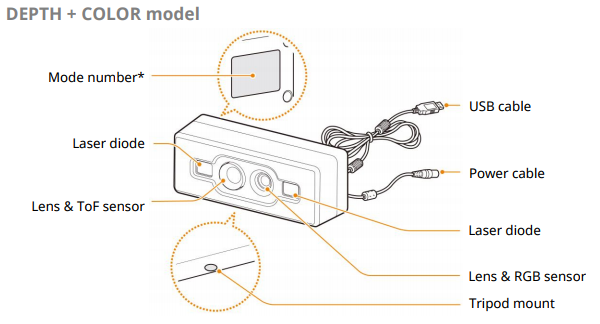
\includegraphics[width=0.6\textwidth]{cube_eye}
	\caption{beschriftetes Bild des Sensors, aus der User Manual des Herstellers}
	\label{cube_eye_sensor}
\end{figure} \par
Einen weiteren wichtigen Teil des Projekts stellen 3D-Audio Kopfhörer dar. Diese können den Eindruck
erzeugen, dass sich eine Tonquelle im dreidimensionalen
Raum befindet bzw. sich bewegt. Dieses Verfahren benutzen wir, um dem Träger des Geräts einen Eindruck
davon zu geben, in welcher Richtung sich ein Objekt befindet.\par 
Die dritte Komponente ist ein Laptop, der später durch einen kleineren Computer, wie z.B. ein \enquote{Raspberry Pi}
ersetzt werden soll. Dieser ist mit Kopfhörern und dem ToF-Sensor 
verbunden und führt unser Programm aus.\par 
Zusammen ergeben die drei Bestandteile (und ein externer Bleiakku für die Tof-Kamera) einen mobilen Prototypen, den wir zum Ausstellungstag vorführen werden. Die Technik befindet sich dabei in einem Rucksack und der Sensor wird mit einem
umgebauten Stirnband am Kopf befestigt. 
\begin{figure}[H]
	\centering
	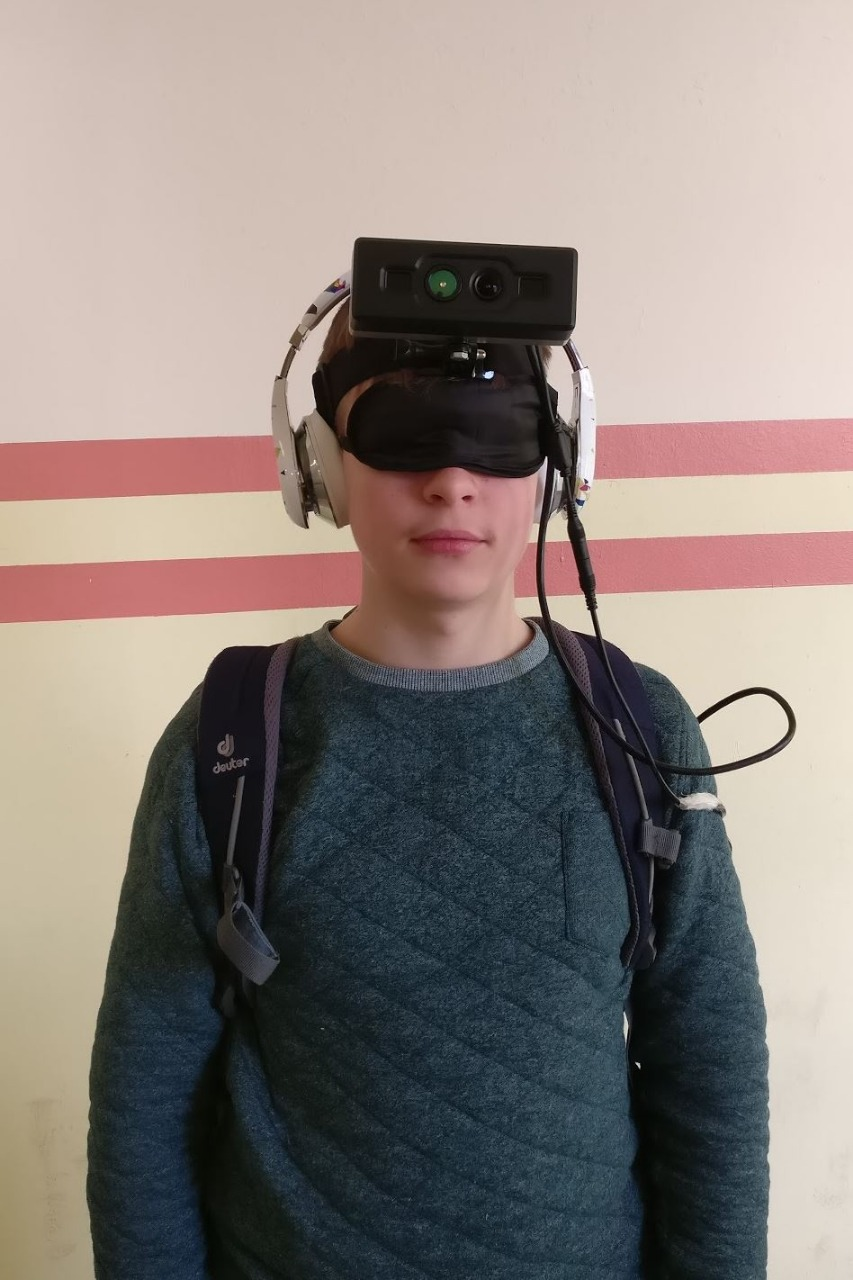
\includegraphics[width=0.4\textwidth]{device}
	\caption{Aufbau des portablen Prototyps}
	\label{dosuas_device}
\end{figure} 

\subsection{Softwarestruktur}

Das Programm ist in C++ geschrieben, weil die API des ToF Sensors C++ erfordert und C++ eine schnelle, objektorientierte und betriebssystemunabhängige Sprache mit vielen Möglichkeiten ist. Momentan wird das Programm
auf Windows 10 32-Bit mit Visual Studio 2017 entwickelt.
Wir verwenden folgende Libraries:
\begin{enumerate}
	\item \textit{MTF API} - eine Schnittstelle mit der man den Cube Eye Sensor ansteuern kann
	\item \textit{SFML} - eine einfache Multimedia Bibliothek zum Abspielen von 3D-Sounds und generieren von 
	Tönen
\end{enumerate} 
Die Software selbst besteht im Moment aus 3 Modulen, die sich aber bis zur Ausstellung noch verändern 
können.
\begin{enumerate}
	\item \textit{sensorReader.cpp} - ein Modul, das die Schnittstelle zum ToF Sensor benutzt, um Daten zu 
	lesen und in eine Struktur für die weitere Verarbeitung zu bringen
	\item \textit{imageProcessor.cpp} - ein Modul zum Filtern und Umwandeln der 3D-Bilder in Anweisungen zum 
	Tonabspielen (Frequenzen und deren Spieldauer, Position der Tonquellen, Lautstärke etc.)
	\item \textit{audioPlayer.cpp} - ein Modul, welches zu den Anweisungen passende Töne generiert und abspielt
\end{enumerate}
Den Sourcecode finden Sie auf https://github.com/YpsilonZett/Dosuas.
Im folgenden beschreiben wir den Ablauf des Programms und die Unterschiede der einzelnen Modi.

\subsection{Vorverarbeitung}

Zuerst macht die Kamera ein Bild und stellt es als 2D Matrix von 320$\times$240 (=76800) natürlichen Zahlen dar.
In diesem Tiefenbild gibt jeder Pixel den Abstand zur nächsten lichtreflektierenden Region in mm an. 
Dadurch erscheint eine gerade Fläche direkt vor dem Sensor jedoch auf dem Bild als nach außen gekrümmt, 
weil das vom Sensor gesendete Infrarotlicht zu den Seiten der Fläche (und zurück) ein bisschen länger
braucht als zur Mitte. Wegen der kugelförmigen Ausbreitung der Lichtstrahlen von der Kameralinse hat das
Bild außerdem ein Polarkoordinatensystem\footnote{jede Koordinate gibt eigentlich einen Winkel zwischen
	0$^{\circ}$ und 75$^{\circ}$ (horizontal) oder 0$^{\circ}$ und 60$^{\circ}$ (vertikal) an,
	 weil der Sensor ein Sichtfeld von 75$^{\circ}\times$60$^{\circ}$ hat}, mit dem wir nicht
gut weiterarbeiten können. Um das Problem der Verzerrung zu beheben und das Bild in ein kartesisches
Koordinatensystem umzurechnen, verwenden wir einen Undistortion\footnote{in unserem Fall einen
	vom Hersteller mitgelieferten, den man direkt in der Sensorkonfiguration einstellen kann} Algorithmus.
Hier sieht man ein verzerrtes Bild (Darstellung als Punktwolke\footnote{Punktwolken sind ggf. geordnete Mengen
von Punkten mit x-, y- und z-Koordinate}), vor der Anwendung des Undistortion-Algorithmus.
\begin{figure}[H] \label{distorted_pointcloud_img}
	\centering
	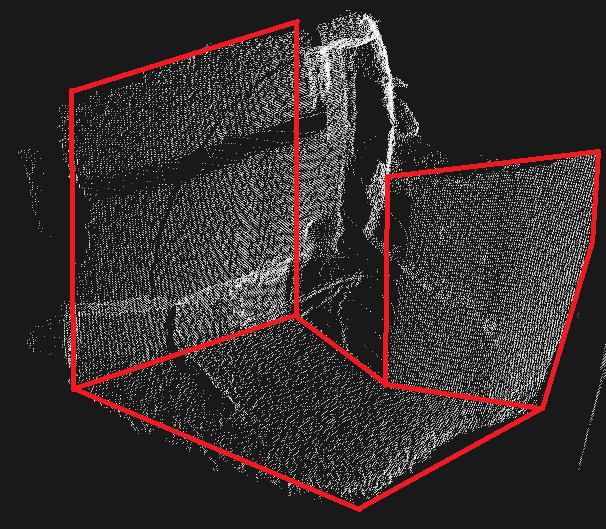
\includegraphics[width=0.6\textwidth]{no_undistortion2}
	\caption{verzerrte Punktwolke mit Messfehlern}
\end{figure}
Wie in Abb. \ref{distorted_pointcloud_img} zu sehen ist, wirkt ein ebene Fläche wie ein Teil der Oberfläche einer Kugel. Mit Rot sind hier ungefähr die echten Flächen (ohne Verzerrung) markiert, damit man die 
Abweichung vom Original sehen kann. Dieser Raum enthält eine Menge 
Flächen und ist relativ einfach aufgebaut. Deshalb eignet er sich gut als Testumgebung.
\begin{figure}[H]
	\centering
	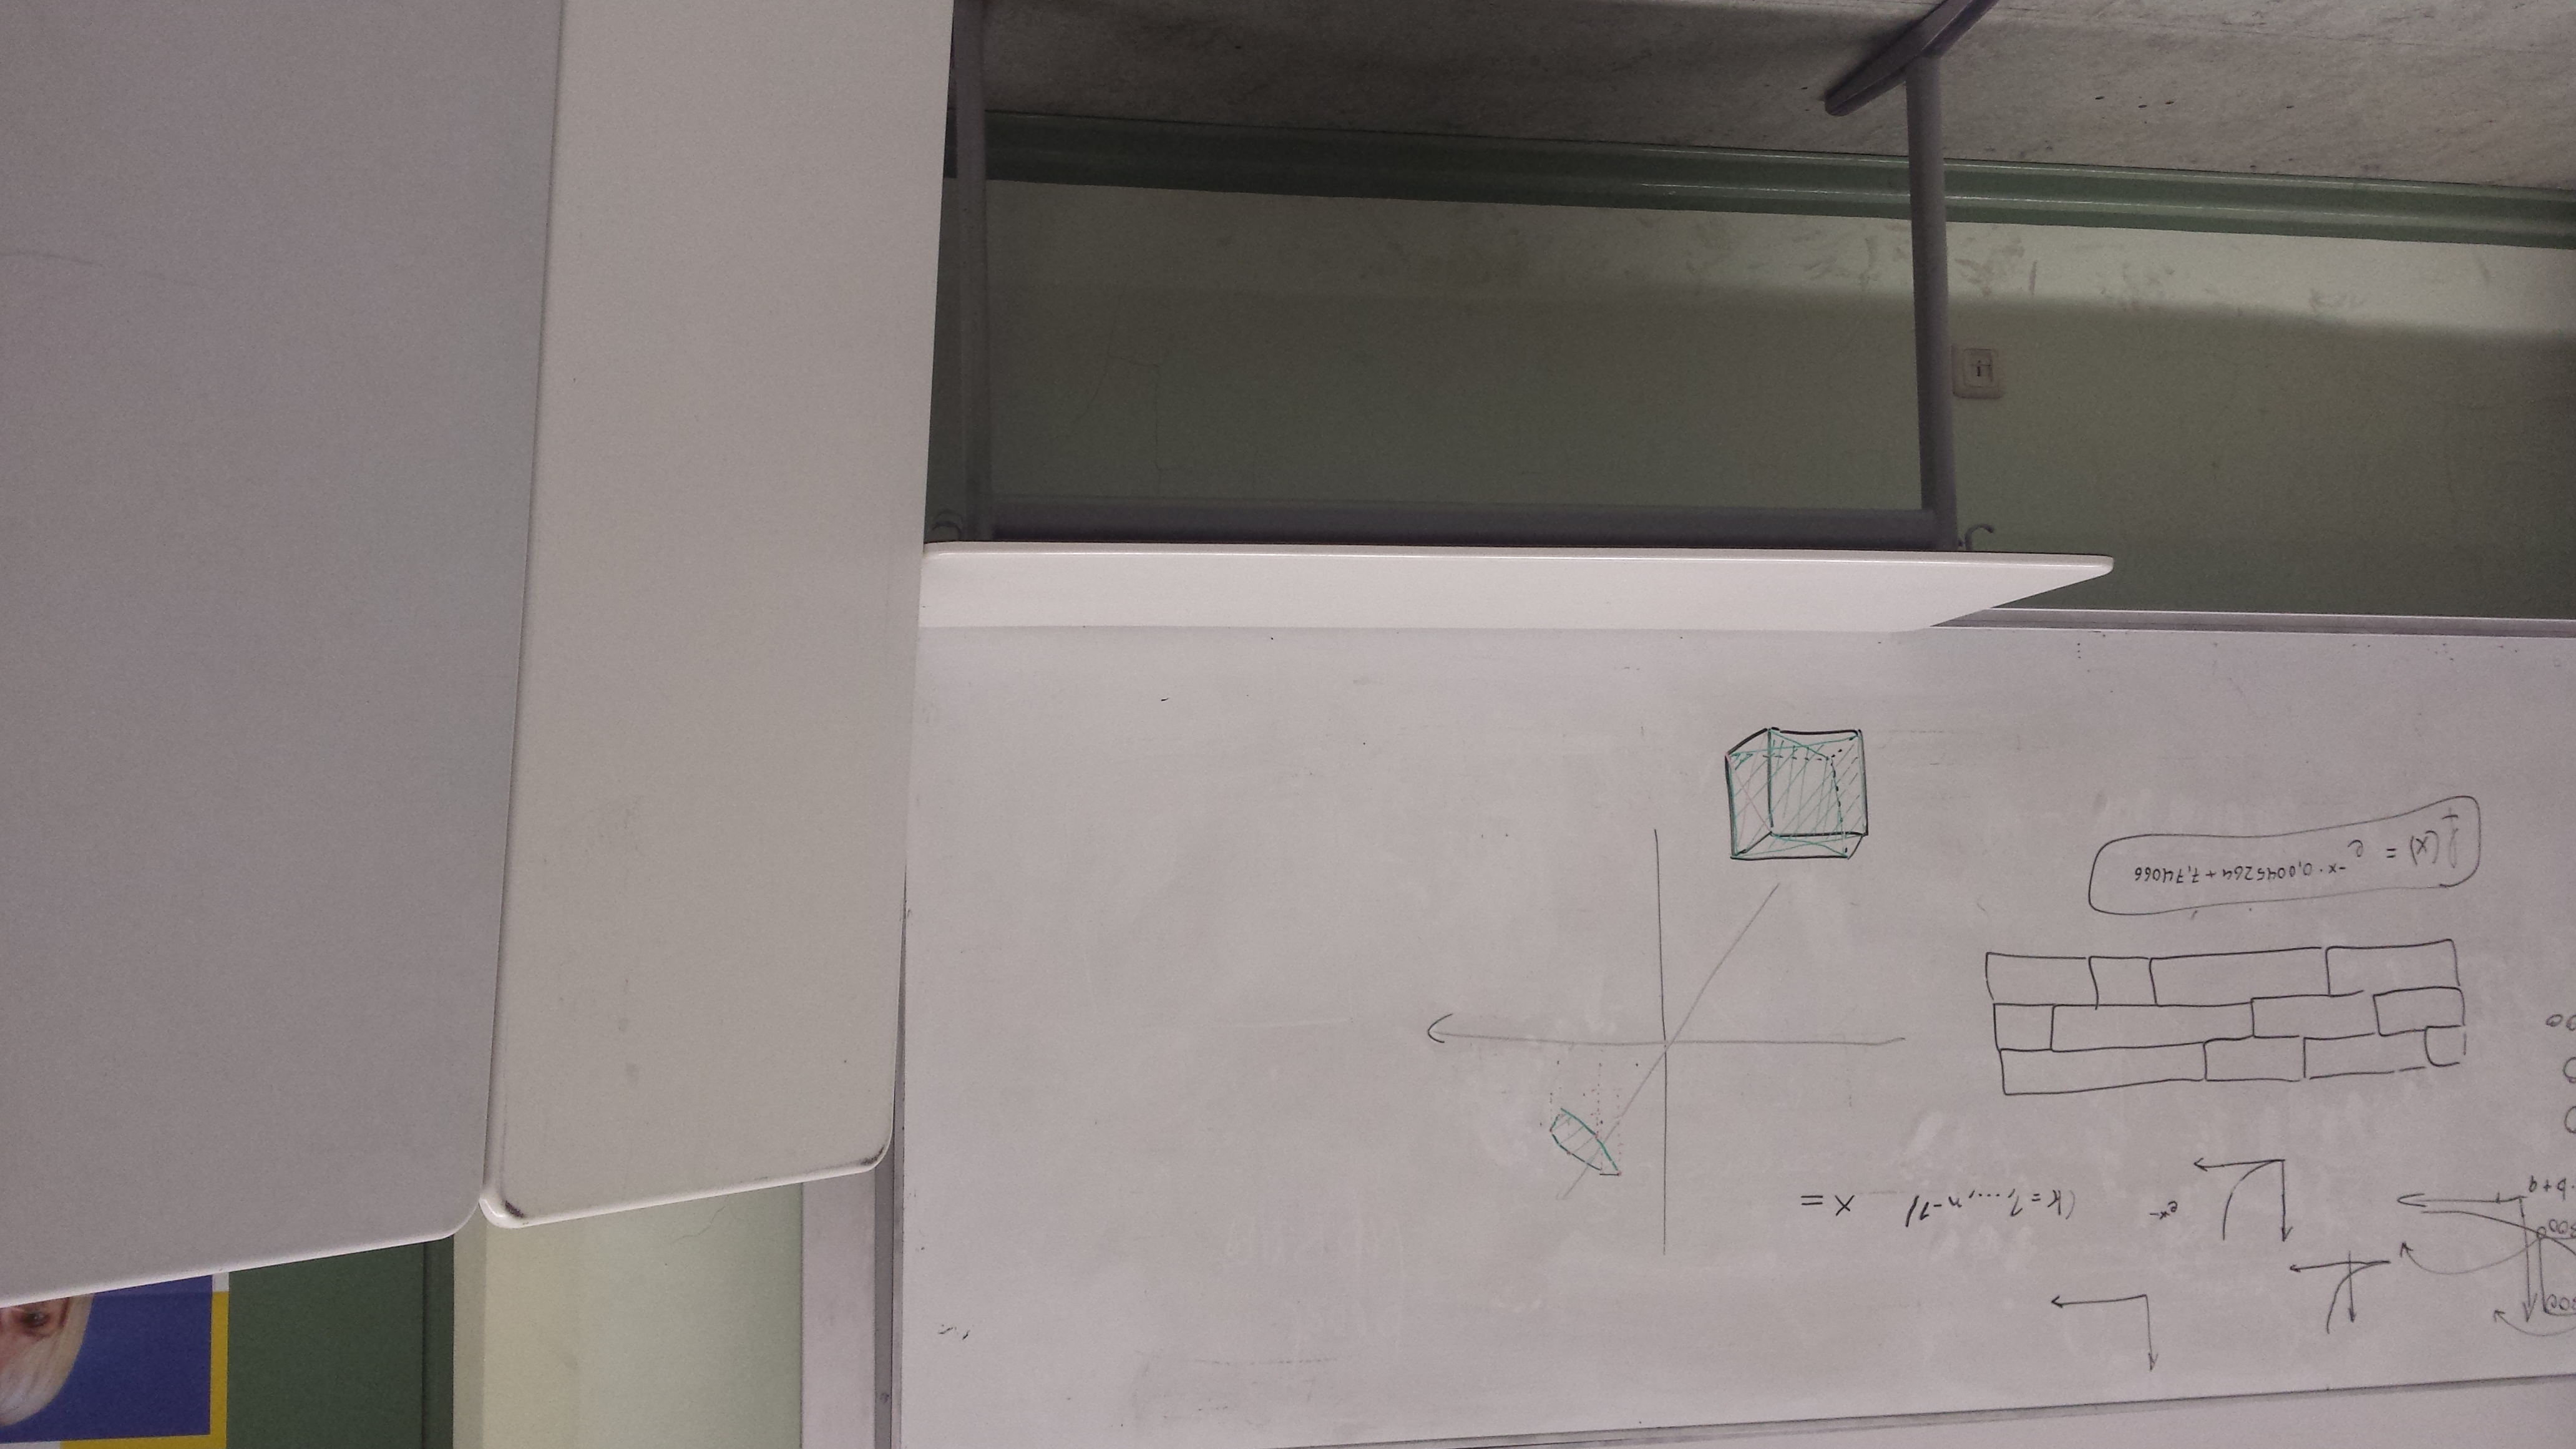
\includegraphics[angle=180,width=0.6\textwidth]{20180125_171703}
	\caption{Kamerabild des Raumes aus Abb. \ref{room_at_school}}
	\label{room_at_school}
\end{figure} \par
In der nächsten Abbildung (Abb. \ref{before_filtering}) sieht
man die Aufnahme des selben Zimmers, in der die Wände gerade erscheinen. Durch die Visualisierung hat man
den Eindruck, dass die Flächen Streifen (sogenannte Moir\'{e} Muster) enthalten. Das liegt jedoch an der
Visualisierung und hat nichts mit dem eigentlichen Bild zu tun. Die dünnen Linien rechts im Bild sind Punkte
mit der z-Koordinate 0, was Messfehler anzeigt. Diese entstehen, wenn etwas zu nah, zu weit oder zu stark
reflektierend ist, um von Sensor erkannt zu werden. Im späteren werden sie entfernt.
\begin{figure}[H]
	\centering
	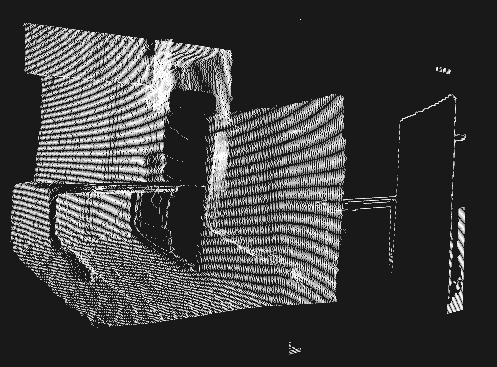
\includegraphics[width=0.6\textwidth]{before_filtering}
	\caption{algorithmisch korrigierte Punktwolke ohne Verzerrung}
	\label{before_filtering}
\end{figure} 

\subsection{Einfacher Modus}

Der einfache Modus stellt eine Art horizontalen Schnitt durch das Bild als Ton dar. Dieser enthält Informationen
über die Position auf der x-Achse (links, rechts, etc.) und Entfernung einer Region, Welche der Nutzer verwenden kann,
um sich grob zu orientieren. Die x-Position wird mit 3D-Audio dargestellt. Mit den richtigen Kopfhörern und etwas Übung
kann man sehr genau bestimmen, in welche Richtung und wie weit weg sich eine Tonquelle befindet. Die Entfernung wird
durch die Tonhöhe angegeben, wobei etwas Nahes als hoher Ton und etwas weit entferntes als tiefer Ton gehört wird.
Nach einigem Experimentieren stellte es sich heraus, dass Töne zwischen 300 und 2300 Hz sich angenehm anhören und auch
längere Zeit (bei angemessener Lautstärke) ertragen lassen. \par 
Die Kombination aus Position und Frequenz ermöglicht es, im
einfachen Modus einen \enquote{Querschnitt} durch das Bild darzustellen. Es ist jedoch nicht besonders hilfreich, 
den Querschnitt an einer festgelegten Höhe durchzuführen. Wenn man z.B. im Raum aus Abb. \ref{room_at_school} den Schnitt im oberen Viertel des Bildes durchführen würde, würde er keine Informationen über den Tisch, der näher ist, als
die Wand, enthalten. Daher teilen wir das Bild in Spalten, nehmen aus jeder Spalte den \enquote{nächsten} Voxel 
(mit der kleinsten z-Koordinate), generieren einen Ton für ihn und setzten diese Töne zu einem Ton zusammen. \par
Bei so einem Ton hat man den Eindruck, dass die Tonquelle gleichmäßig von links nach rechts wandert und dabei ständig
die Tonhöhe ändert. Wir nennen so einen Ton \enquote{Radar Swipe}, weil er einem Radarscan ähnelt.
Um Wände, Türen, Menschen und große Gegenstände (z.B. Schränke oder Tische) zu erkennen reichen diese Informationen völlig aus. So kann man also in den meisten Räumen umher laufen und sich relativ frei bewegen.\par
Zum Beispiel könnte ein Ton, der in der linken Bildhälfte hoch anfängt, dann langsam tiefer wird und 
in der rechten Bildhälfte gleich bleibt, eine schräge Wand darstellen, die in einiger Entfernung in eine
zum Nutzer parallele Wand übergeht. So ein einfaches Beispiel kommt zwar selten vor, und meistens gibt es
noch eine Menge Störgeräusche, aber näheres dazu im Abschnitt \ref{testsAndResults}.\par 
Momentan beträgt die Dauer zum Abspielen eines Bildes fünf Sekunden, gefolgt von einer halben Sekunde 
Pause. Bis zum Wettbewerb wollen wir die Dauer noch verkürzen, jedoch erfordert das ein gewisses 
Training, weil der Mensch üben muss, mehr Informationen in kürzerer Zeit zu verarbeiten. Zusammen mit 
einer Verkürzung der Pausen zwischen Aufnahmen hoffen wir die Zeit für einen Programmzyklus auf ungefähr
zweieinhalb bis vier Sekunden zu reduzieren. 

\subsection{Fortgeschrittenen-Modus}

In diesem Modus wird das gesamte Bild, also ein dreidimensionales Modell der Umgebung, als Töne dargestellt. 
Der Nutzer soll ein genaues Gefühl dafür bekommen, welche Umrisse einzelne Gegenstände haben und so die Form, Entfernung und Ausrichtung aller mittelgroßen und großen Objekte in einem Raum bestimmen können. \par 
Wir Menschen können an einem Ton im Wesentlichen drei
Eigenschaften ausmachen: Lautstärke, Position und Höhe. Wir reden hier von reinen Sinuswellen, da diese momentan für 
das Projekt ausreichen. Später kann man noch kompliziertere Töne einbauen, aber das würde das Lernen erschweren
und ist momentan nicht nötig. Die drei genannten Eigenschaften sollte man, wenn man mit dem Gehör viele Informationen
verarbeiten will, alle nutzen. Es ist wichtig anzumerken, dass Tonhöhe und Lautstärke viel genauer wahrgenommen werden
können, als die Position, und wir sie daher mehr verwenden. \par 
Die 3D-Audio Position übernimmt hier wieder die Funktion der x-Achse im Bild. Wie beim vorherigen Radar Swipe bewegt
sich eine Tonquelle gleichmäßig vom linken bis zum rechten Rand des Sichtfeldes. Wieder wird das Bild in Spalten 
unterteilt, diesmal jedoch in sehr viel niedriger aufgelöste. Eine Spalte besteht nur aus 24 Voxeln.
Jedem dieser Voxel wird nun eine Frequenz zugeordnet, die der Höhe im Bild (y-Koordinate) entspricht.
Voxel am unteren Bildrand bekommen eine Frequenz von 220 Hz und Voxel am oberen Rand eine von 880 Hz. Die 24 
Pixel-Frequenzen bilden genau zwei Oktaven, wobei die Frequenzen so ausgesucht sind, dass sie harmonisch zueinander
passen. Jedem der Pixel wird nun eine Lautstärke zugeordnet, die die Tiefe (z-Koordinate) wiedergibt. Eine geringe
z-Koordinate entspricht einem lauten Ton. Dies ist intuitiv logischer, da nähere Objekte meist lautere Töne abgeben.
\par 
Beim Abspielen des Tones erklingen alle Pixel einer Spalte gleichzeitig und bilden so einen Akkord aus 24 Tönen 
mit unterschiedlichen Lautstärken. Alle diese Akkorde (es gibt 32 Spalten) werden hintereinander abgespielt, während
sich die Tonquelle entsprechend der x-Koordinate einer Spalte bewegt. Zusammen bilden sie eine komplizierte Melodie.
Zusammengefasst: x-Koordinate $\hat{=}$ 3D-Audio Position, y-Koordinate $\hat{=}$ Frequenz und z-Koordinate $\hat{=}$ Lautstärke.

\subsubsection{Warum ist das sinnvoll?}

Wir denken, dass dieses Verfahren eine sehr gute Modellierung von 3D-Daten durch Töne ist. Wir wollen hier einige 
Fragen beantworten, die man sich unsere Wahl betreffend stellen könnte und unsere Entscheidungen begründen.
\begin{enumerate}
	\item \textbf{Warum benutzen wir die y- und z-Koordinate der 3D-Audio Tonquellen nicht?} - \textit{Man könnte die
	räumliche Position der 3D-Audio Tonquelle benutzten, um genauere Informationen über die Position eines
	Objektes anzuzeigen. Bei unseren Versuchen ist uns aber aufgefallen, dass es sehr schwer ist, die y-Koordinate einer 3D-Audio Quelle auch nur annähernd genau zu bestimmen. Um eine auf der z-Achse verschobene Tonquelle 
	darzustellen benötigt man die Lautstärke, die wir aber bereits für etwas anderes verwenden. Deshalb
	bleiben wir beim einfachen Stereo\footnote{es stellte sich übrigens dabei heraus, dass wir auf aufwändige
	3D-Audio Kopfhörer hätten verzichten können, weil normale Stereo-Kopfhörer gereicht hätten, aber das konnten wir vorher nicht wissen}.}
	\item \textbf{Warum werden Frequenzen für die Höhe im Bild und nicht für die Entfernung verwendet?} - \textit{Würden wir Frequenzen für die Entfernung verwenden, müssten wir die Lautstärke verwenden, um Höhe auf dem Bild darzustellen. Dann wären aber nur die oberen Reihen des Bildes 
	hörbar, weil das Gehör sich bei vielen Tönen auf die lautesten konzentriert. Diese Eigenschaft nutzen wir bei 
	unserer Version viel besser aus, 
	um das Gehirn dazu zu bringen, nähere Regionen besser zu erkennen, da diese wichtiger sind.}
	\item \textbf{Wie kann das Gehör mit den vielen verschiedenen Frequenzen umgehen?} - \textit{Wie bereits gesagt, filtert das 
	Gehör bei vielen Tönen die heraus, die uns am wichtigsten erscheinen. Man bezeichnet dieses Phänomen als Cocktailparty-Effekt 
	oder selektives Hören. Wenn wir uns auf bestimmte Töne konzentrieren (z.B. die Stimme einer Person bei einer Unterhaltung vieler
	Personen) nehmen wir diese bis zu dreimal lauter wahr, als sie eigentlich sind. Bei den von uns erzeugten Akkorden stechen meistens
	zusammengesetzte oder einzelne Töne, die lauter sind als der Rest, heraus. Dadurch konzentrieren wir uns auf sie und nehmen sie noch deutlicher wahr. Mit etwas Übung kann man auch aus einem Akkord von vielen Tönen 
	die einzelnen heraushören und die Höhe so noch deutlicher wahrnehmen.}
\end{enumerate}

\newpage

\section{Praxistests} \label{testsAndResults}

Wir haben DOSUAS in verschiedenen Umgebungen getestet und werden Ihnen am Ausstellungstag einen Prototypen vorführen.

\subsection{Einfacher Modus}

Es stellte sich heraus, dass sich zum Üben der Handhabung des Gerätes mittelgroße Räume mit einfachen
Formen besser eigenen. Die Räume dürfen aber nicht zu groß sein, weil der Sensor eine maximale Reichweite
von 5,3 Metern hat. Auch in zu kleinen Räumen eignet sich das Gerät nicht, denn der Sensor hat eine  Mindestreichweite von 0,8 Metern. Am Anfang sind Räume ohne viele kleine Objekte und mit großen 
Flächen wie Wänden einfacher, weil die Töne gleichmäßiger sind.
Hier sieht man einen anderen Raum, an dessen Beispiel wir die Töne beschreiben wollen, die man
mit unserem Gerät hört.
\begin{figure}[H]
	\centering
	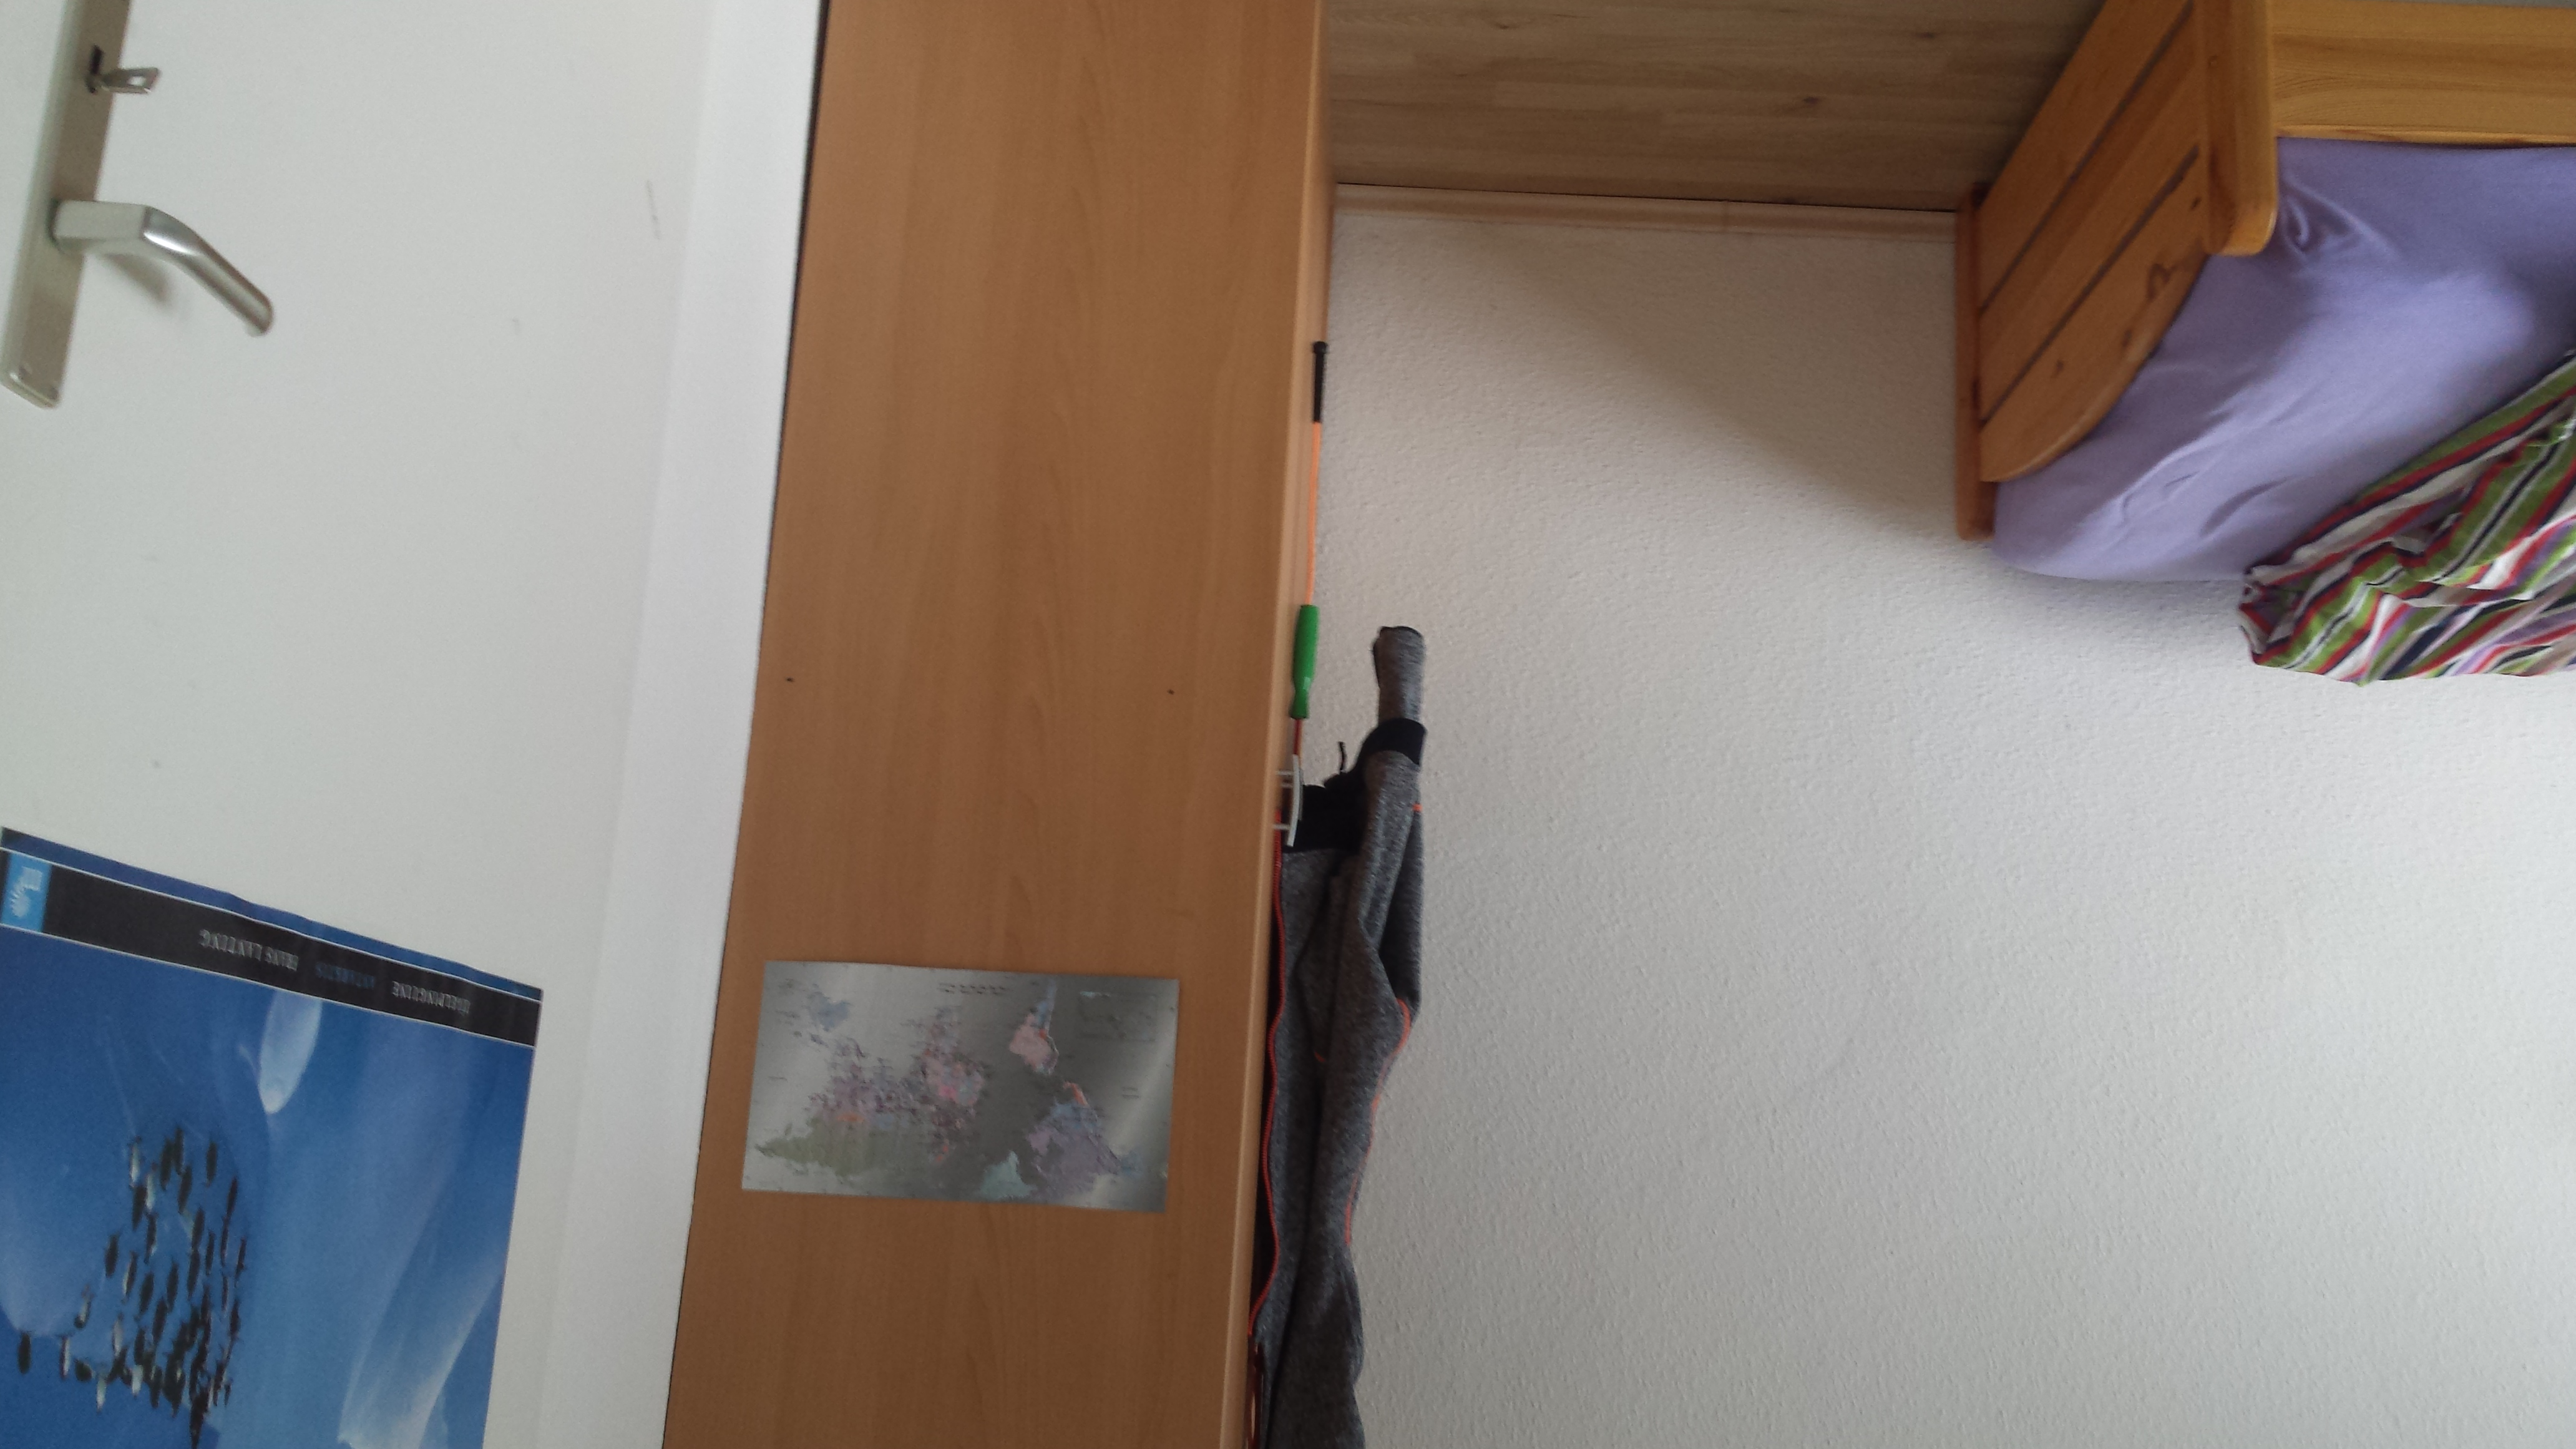
\includegraphics[angle=180,width=0.5\textwidth]{20180120_114953}
	\caption{Kamerabild eines anderen Raumes}
	\label{normal_picture}
\end{figure} \par
Man hört beim Betrachten dieses Raumes einen Ton, der ungefähr eine halbe Sekunde die Frequenz (von ca. 550 Hz) nicht verändert und sich so anhört, als würde er von links kommen. Dieser Ton wird durch das Bett
erzeugt. Als nächstes wird der Ton über ungefähr eine halbe Sekunde gleichmäßig tiefer (bis auf 340 Hz), 
jetzt ist unsere virtuelle Tonquelle an der Wand des Raumes angekommen. Der Ton steigt nun über $1\frac{1}{2}$ Sekunden sehr langsam an (bis ca. 360 Hz), denn die Wand hat eine leichte Neigung. 
Nun hört man eine Art Sprung, bei dem der Ton ruckartig von 360 Hz zurück auf 550 Hz wechselt. An solchen Auffälligkeiten kann man Kanten, Öffnungen oder spitze Gegenstände erkennen, was sehr wichtig für Blinde
ist. Dieser Ton repräsentierte nämlich den Übergang von der Wand zum Schrank, der weiter vorne ist. Außerdem hört
man die virtuelle Tonquelle in diesem Moment direkt in der Mitte des Hörfeldes, was dem Nutzer anzeigt, das sich
die Kante fast genau vor ihm befindet. Über ungefähr eine Sekunde bleibt die Tonhöhe wieder gleich, nur die Position
verändert sich; man hört die Fläche des Schranks. Über die restlichen $1\frac{1}{2}$ Sekunden steigt der Ton mit 
gleichbleibender Geschwindigkeit an und die Tonquelle wandert nach rechts.
Hier hört man die Tür und am Ende eine kurze \enquote{Spitze}, die die Türklinke darstellt. Am Ende hat der Ton
eine Frequenz von ca. 790 Hz.\par 
Wir hoffen, dass Sie sich nun ein Bild davon machen können, wie sich die Welt mit DOSUAS anhört. Nach einem
halbstündigen Training mit dem Gerät waren unsere Testpersonen\footnote{Yorick Zeschke, Jonas Wanke, Petra Zeschke und Peter Kreißig} in der Lage (natürlich mit verbundenen Augen) in Schulräumen und Gängen
Wände und Türen zu erkennen, deren Ausrichtung und Entfernung sie beschreiben konnten, ohne sie gesehen zu haben.
Außerdem konnten sie sagen, ob eine Tür offen, halboffen oder geschlossen ist. Nach einer weiteren halben Stunde
war es ihnen möglich Menschen, Tische, Schränke und deren ungefähre Ausrichtung zu bestimmen. \par
Wir haben bereits einige wiederkehrende Muster gefunden, die auf bestimmte Objekte in einem Raum hindeuten. 
\begin{figure}[h]
	\begin{tabular}{| p{0.4\textwidth} | p{0.5\textwidth} |}
		\hline
		Objekt & Beschreibung des Tons \\ \hline
		Wand oder große Fläche & verändert gleichmäßig und ununterbrochen seine Tonhöhe \\ \hline
		Kante, Ecke, sehr steile Fläche oder spitzer Gegenstand & \enquote{Sprung} von einer Tonhöhe zu einer 
		anderen \\ \hline
		Tür, Öffnung oder Loch & gleichmäßiger Ton (z.B. Wand), dann Sprung (Kante), wieder gleichmäßiger Ton
		(z.B. Gang hinter der Tür), noch ein Sprung und dann wieder ein gleichmäßiger Ton (Wand geht weiter) \\ \hline 
		Mensch oder Säule & gleichmäßiger Ton (z.B. Wand), dann \enquote{kreisförmiger}\footnotemark Ton, dann wieder gleichmäßiger Ton \\ \hline
		unregelmäßiges Objekt (z.B. Gardrobe mit Kleidung oder Computer auf einem Tisch) & zitternd\footnotemark erscheinender Ton \\ \hline 
	\end{tabular}
\end{figure} \par
\footnotetext{Intuitiv würde man so einen Ton wahrscheinlich
	als kreisförmig beschreiben. Die Frequenzänderung kann durch eine nach unter geöffnete gestauchte Parabel angenähert werden.}
\footnotetext{weil der Ton schnell zwischen verschiedenen Frequenzen wechselt} 
Wir wollen das Gerät noch mit
anderen Leuten testen und sehen, wie schnell jemand lernt, damit umzugehen. Wir vermuten, dass man nach einigen 
Tagen Selbsttraining im Stande ist, ohne Hilfe durch noch nie gesehene Räume zu gehen, ohne dabei irgendwo an zu
stoßen und den Weg nach draußen wieder zu finden. Längeres Üben oder technische Verbesserungen bieten ungeahnte
Möglichkeiten. Doch das Gerät ist und bleibt momentan nur ein Prototyp. 

\subsection{Fortgeschrittenen-Modus}

Wir sind im Moment dabei den Fortgeschrittenen-Modus mit verschiedenen Leute zu testen und die Orientierung damit zu üben. Bis jetzt
ist es uns gelungen mit dem Fortgeschrittenen-Modus ein Orientierungsvermögen zu erreichen, das ungefähr so gut ist, wie beim einfachen
Modus. Bis zum Wettbewerb werden wir aber noch weiter Üben und den Fortgeschrittenen-Modus anpassen, weiterentwickeln und besser testen.
Die Testergebnisse werden wir Ihnen dann präsentieren.

\newpage

\section{Diskussion}

Im folgenden wollen wir kurz diskutieren, was wir für das Projekt planen und inwiefern man das
Gerät benutzten und weiterentwickeln kann und sollte. Außerdem fassen wir die durch die Entwicklung und Forschung am Projekt DOSUAS gewonnenen Erkenntnisse im Fazit zusammen.

\subsection{Ausblick}

Es gibt noch sehr viele Möglichkeiten das Projekt weiterzuentwickeln. Einige vielversprechende,
möchten wir hier auflisten. Die Entwicklungen sind nach ihrer Schwierigkeit und Wichtigkeit geordnet. Einige sind auch nur Ideen.
\begin{enumerate}
	\item Verbesserung der Genauigkeit, z.B durch ein größeres Frequenzspektrum
	\item Entwickeln eines Echtzeit-Modus, um das Sehen zu beschleunigen
	\item Einbauen von Texterkennung, sodass das Programm Texte vorlesen kann, die nicht in Braille geschrieben sind
	\item Einbauen von Gesichts- und Objekterkennung, z.B. mit Machine Learning, um bei Bedarf genauere 
	Informationen über Objekte zu sagen (Sprachmodul)
	\item Verkleinern und besser portabel Machen des Geräts, z.B. Laptop durch Raspberry Pi ersetzen oder Programm über
	Handy-App steuern
	\item Benutzen eines auf das Projekt angepassten Sensors und bequemer Machen der Stirnhalterung
\end{enumerate}
Viele der hier aufgezählten Entwicklungen werden wir bis zum Wettbewerb wahrscheinlich nicht 
mehr schaffen. Aber dieser Ausblick dient auch als Ideen für Leute, die nach Jugend forscht 
daran interessiert sind, das Projekt weiter zu entwickeln. 

\subsection{Fazit}

Wir können wir mit Sicherheit sagen, dass erste Schritte wie das Herumlaufen, Orientieren und erkennen einfacher
Objekte in fremden Räumen mit dem jetzigen Stand möglich sind. Der Fortgeschrittenen-Modus bietet sogar noch mehr 
Möglichkeiten und genaueres Verständnis der Umgebung.
Wirklich \enquote{Sehen} können Leute mit dem Gerät noch nicht und der Weg bis dahin ist noch weit.
Aber etwas ebenfalls sehr wichtiges
ist bereits möglich: Erkennen. Mit DOSUAS kann man sich im Raum orientieren, Strukturen, Formen und Entfernungen
mittelgroßer bis großer Objekte erkennen und sich ein relativ genaues Bild von der Umgebung machen. 
Also tut das Gerät genau das, was sein Name sagt, es ist ein Gerät zur Orientierung im Raum mithilfe von Audio
Signalen, ein \enquote{\textbf{D}evice for \textbf{O}rientation in \textbf{S}pace \textbf{U}sing 
	\textbf{A}udio \textbf{S}ignals}.\par 
Das Gerät ist natürlich kein Ersatz für menschliches Sehen, aber das war am Anfang der Entwicklung
auch gar nicht beabsichtigt. Das Projekt DOSUAS sollte eine Hilfestellung für Blinde sein, die ihnen das Leben einfacher macht. Kleine oder komplizierte Gegenstände kann man mit unserem jetzigen Sensor nicht besonders gut erkennen. Das muss man aber auch nicht, denn dazu besitzen wir Menschen den Tastsinn, der wesentlich genauer ist,
als jeder 3D-Sensor der heutigen Zeit. Auch sonst ist es nicht beabsichtigt, sich auf 
ein Gerät wie dieses zu verlassen. Man kann alltägliche Prozesse mit DOSUAS einfacher machen.\par
Wir hoffen, dass dieses oder ähnliche Projekte mehr blinde Menschen dazu motiviert, sich nicht 
mit ihrer Behinderung wie mit einer Last abzumühen, sondern Geräte oder Techniken
wie z.B. menschliche Echoortung, zu verwenden, um nicht mehr auf ständige Hilfe angewiesen 
zu sein und selbständiger zu werden. Wie Daniel Kish in einem TED-Talk\footnote{https://www.ted.com/talks/daniel\_kish\_how\_i\_use\_sonar\_to\_navigate\_the\_world} sagte, 
empfindet er Blindheit nicht als Problem, sondern als Eigenschaft, die ihn von anderen Menschen
unterscheidet. Diesem Beispiel sollten unserer Meinung nach mehr Blinde folgen.\par 
Vielleicht wird DOSUAS irgendwann die Grundlage für ein weiteres
Forschungsprojekt sein, das es blinden Menschen vollständig ermöglicht zu sehen. Bis dahin
warten wir gespannt und versuchen mit unserem Projekt den Grundstein dafür zu legen. 

\newpage

\end{document}